\documentclass[a4paper, 12pt]{article}

%%% Работа с русским языком
\usepackage{cmap}					% поиск в PDF
\usepackage{mathtext} 				% русские буквы в формулах
\usepackage[T2A]{fontenc}			% кодировка
\usepackage[utf8]{inputenc}			% кодировка исходного текста
\usepackage[russian]{babel}	% локализация и переносы

%%% Дополнительная работа с математикой
\usepackage{amsmath,amsfonts,amssymb,amsthm,mathtools} % AMS
\usepackage{icomma} % "Умная" запятая: $0,2$ --- число, $0, 2$ --- перечисление

%% Номера формул
%\mathtoolsset{showonlyrefs=true} % Показывать номера только у тех формул, на которые есть \eqref{} в тексте.

%% Шрифты
\usepackage{euscript}	 % Шрифт Евклид
\usepackage{mathrsfs} % Красивый матшрифт

%% Поля
\usepackage[left=2cm,right=2cm,top=2cm,bottom=2cm,bindingoffset=0cm]{geometry}

%% Русские списки
\usepackage{enumitem}
\makeatletter
\AddEnumerateCounter{\asbuk}{\russian@alph}{щ}
\makeatother

%%% Работа с картинками
\usepackage{graphicx}  % Для вставки рисунков
\graphicspath{{images/}{images2/}}  % папки с картинками
\setlength\fboxsep{3pt} % Отступ рамки \fbox{} от рисунка
\setlength\fboxrule{1pt} % Толщина линий рамки \fbox{}
\usepackage{wrapfig} % Обтекание рисунков и таблиц текстом

%%% Работа с таблицами
\usepackage{array,tabularx,tabulary,booktabs} % Дополнительная работа с таблицами
\usepackage{longtable}  % Длинные таблицы
\usepackage{multirow} % Слияние строк в таблице

%% Красная строка
\setlength{\parindent}{2em}

%% Интервалы
\linespread{1}
\usepackage{multirow}

%% TikZ
\usepackage{tikz}
\usetikzlibrary{graphs,graphs.standard}

%% Верхний колонтитул
\usepackage{fancyhdr}
\pagestyle{fancy}

%% Перенос знаков в формулах (по Львовскому)
\newcommand*{\hm}[1]{#1\nobreak\discretionary{}
	{\hbox{$\mathsurround=0pt #1$}}{}}

%% Мои дополнения
\usepackage{float} %Добавляет возможность работы с командой [H] которая улучшает расположение на странице
\usepackage{gensymb} %Красивые градусы
\usepackage{graphicx}               % Импорт изображений
\usepackage{caption} % Пакет для подписей к рисункам, в частности, для работы caption*

% подключаем hyperref (для ссылок внутри  pdf)
\usepackage[unicode, pdftex]{hyperref}

%%% Теоремы
\theoremstyle{plain}                    % Это стиль по умолчанию, его можно не переопределять.
\renewcommand\qedsymbol{$\blacksquare$} % переопределение символа завершения доказательства

\newtheorem{theorem}{Теорема}[section] % Теорема (счетчик по секиям)
\newtheorem{proposition}{Утверждение}[section] % Утверждение (счетчик по секиям)
\newtheorem{definition}{Определение}[section] % Определение (счетчик по секиям)
\newtheorem{corollary}{Следствие}[theorem] % Следстиве (счетчик по теоремам)
\newtheorem{problem}{Задача}[section] % Задача (счетчик по секиям)
\newtheorem*{remark}{Примечание} % Примечание (можно переопределить, как Замечание)
\newtheorem{lemma}{Лемма}[section] % Лемма (счетчик по секиям)

\begin{document}
    \newcommand{\HRule}{\rule{\linewidth}{0.7mm}} % Defines a new command for the horizontal lines, change thickness here
	
	\begin{center}
		\large\textbf{Московский Физико-Технический Институт}\\ % Name of your university/college
		\large\textbf{(государственный университет)}
	
		\vfill
		
		\Large Лабораторная работа по курсу общей физики № *labnum*\\[0.5cm] % Preambule of your document title
		
		
		\HRule
		\\[0.4cm]
		{ \huge \bfseries *name of your labwork*}% Title of your document
		\\[0.4cm] 
		\HRule
		\\[0.5cm]
		
		\ \\
	\textbf{\large Автор:} \\	
	\large *your name* *groupname*\\ % Your name and something more, your group num for example
		\vfill
		\hspace*{-0.8 cm}
\includegraphics[width=100 pt]{frkt_logo}\\ % logo of your  company/university/college
		\large Долгопрудный, 2021 % location and year
	\end{center}

\newpage
\setcounter{page}{2}
\fancyfoot[c]{\thepage}
\fancyhead[L] {Работа № *labnum*} % some information in page header
\fancyhead[R]{}

    \section*{Цель работы}

    С помощью сцинтилляционного спектрометра исследуется энергетический спектр $\gamma$-квантов, 
    рассеянных на графите. 
    Определяется энергия рассеянных $\gamma$-квантов в зависимости от угла рассеяния, 
    а также энергия покоя частиц, на которых происходит комптоновское рассеяние.

    \section*{Теоретическая чать}

    Эффект Комптона -- увеличение длины волны рассеянного излучения по сравнению с падающим -- интерпретируется как результат упругого соударения двух частиц: $\gamma$-кванта и свободного электрона.
	
	Из закона сохранения 4-имульса для системы <<фотон + электрон>> следует формула для изменения длины волны рассеянного излучения:
	\begin{equation}
		\label{Kompton}
		\tag{$\star$}
		\Delta \lambda = \Lambda_K(1-\cos\theta),
	\end{equation}
	где величина $\Lambda_K = h/(mc) = 2,42 \cdot 10^{-10}$ см называется комптоновской длиной волны электрона.
	
	Из формулы (\ref{Kompton}) следует, что комптоновское смещение не зависит ни от длины волны первичного излучения, ни от рода вещества, в котором наблюдается рассеяние. В общем случае комптоновоское рассеяние происходит на свободных электронах в атоме. Для $\gamma$-квантов с энергией в несколько десятков, а тем более сотен килоэлектрон-вольт, связь электронов в атоме мало существенна, так как энергрия их связи в легких атомах не превосходит нескольких килоэлектрон-вольт, а для большинства электронов еще меньше.
	
	При рассеянии на связанных электронах изменение импульса кванта воспринимается атомом в целом. Посколько масса атома очень велика, переда ча импульса не спровождается сколь-нибудь заметной передачей энергии, и наблюдается несмещенная (по энергии) компонента в спектре рассеянного излучения. Таким образом, рассеяние $\gamma$-квантов на связанных электронах можно рассматривать как упругое столкновение квантов с атомами.
	
	Основной целью данной работы является проверка соотношения (\ref{Kompton}). Применительно к условиям нашего опыта формулу (\ref{Kompton}) следует преобразовать от длин волн к энергиям $\gamma$-квантов. Как нетрудно показать, соответсвующиее выражение имеет вид:
	\begin{equation}
		\label{1-cos}
		\tag{$\star\star$}
		\frac{1}{\varepsilon(\theta)} - \frac{1}{\varepsilon_0} = 1 - \cos \theta.
	\end{equation}

	Здесь $\varepsilon_0 = E_0/(mc^2)$ -- выраженная в единицах $(mc^2)$ энергия $\gamma$-квантов, падающих на рассеиватель, $\varepsilon(\theta)$ -- выраженная в тех же единицах энергия квантов, испытавших комптоновское рассеяние на угол $\theta$, $m$ -- масса электрона.
	
	Заменим в формуле~(\ref{1-cos}) энергию квантов, испытавших комптоновское рассеяние на угол $\theta$, номером канала $N(\theta)$, соответствующего вершине фотопика при указанном угле $\theta$:
	\begin{equation}
		\label{kek}
		\tag{$\star \star \star$}
		\frac{1}{N(\theta)} - \frac{1}{N(0)} = A (1- \cos \theta),
	\end{equation}
	где $A$ -- неизвестный коэффциицент пропорциональности между $\varepsilon(\theta)$ и $N(\theta)$.

    \section*{Эксперементальная установка}

    Источником излучения служит $^{137}$Cs, испускающий $\gamma$-лучи с энергией 662 кэВ. 
    Он помещен в свинцовый контейнер с коллиматором. 
    Сформированный коллиматором узкий пучок $\gamma$-квантов попадает на графитовую мишень.

    \begin{figure}
        \centering
        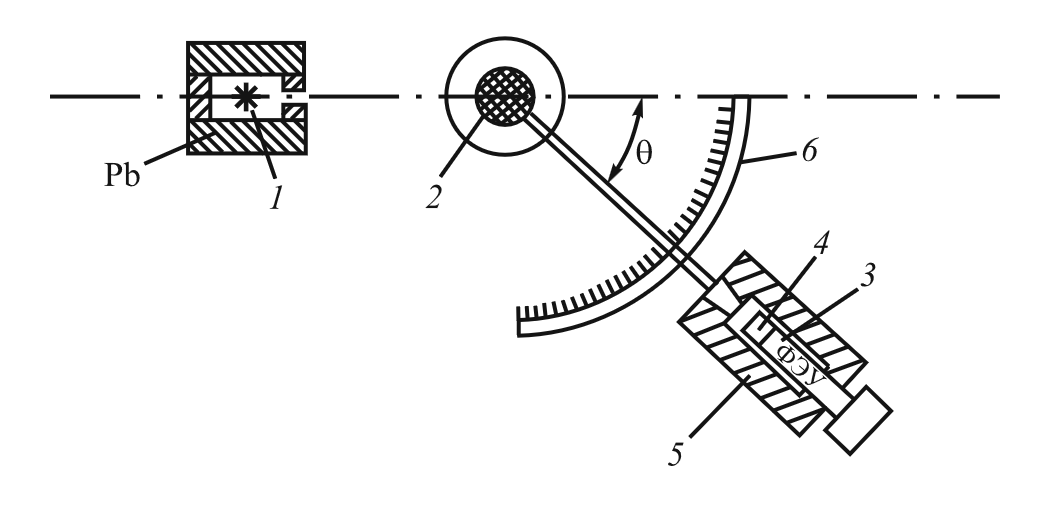
\includegraphics[width=\textwidth]{ust.png}
        \caption{Схема эксперементальной установки}
        \label{fig:ust}
    \end{figure}

    Кванты, испытавшие комптоновское рассеяние в мишени, 
    регистрируются сцинтилляционным счетчиком. 
    Счетчик состоит из фотоэлектронного умножителя 3 (далее ФЭУ) и сцинтиллятора 4. 
    Сцинтиллятором служит кристалл NaI(Tl) цилиндрической формы диаметром 40 мм и высотой 40 мм, 
    его выходное окно находится в оптическом контакте с фотокатодом ФЭУ. 
    Сигналы, возникающие на ФЭУ, подаются на ЭВМ для амплитудного анализа. 
    Кристалл и ФЭУ расположены в светонепроницаемом блоке, укрепленном на горизонтальной штанге. 
    Штанга вместе с этим блоком может вращаться относительно мишени, 
    угол поворота отсчитывается по лимбу 6.

    \section*{Обработка эксперементальных данных}

    В формуле для эффекта Комптона 

    \begin{equation}
        \Delta \lambda = \frac{h}{mc} (1 - \cos \theta)
    \end{equation}

    перейдем от длин волн к энергиям фотонов

    \begin{equation}
        \frac{1}{\varepsilon(\theta)} - \frac{1}{\varepsilon_0} = 1 - \cos \theta
    \end{equation}

    где $\displaystyle \varepsilon(\theta) = \frac{E(\theta)}{mc}$ -- приведенная энергия фотона. 
    При этом $m$ -- масса электрона, соответственно $\varepsilon(0) = \varepsilon_0$ -- 
    энергия фотонов, падающих на рассеиватель.

    Теперь заменим в последней формуле приведенную энергию фотона на номер канала $N$, соответсвующего
    вершине фотопика при указанном угле $\theta$.

    \begin{equation}
        \frac{1}{N(\theta)} - \frac{1}{N(0)} = 1 - \cos \theta
    \end{equation}

    \begin{table}[h!]
    \centering
    \begin{tabular}{|c|c|c|c|c|c|}
    \hline
    $T_{br}$, $^oC$   & $I$, А              & $U$, мВ                & $T$, $^oC$                 & $W$, мВт   & $\varepsilon_W \cdot 10^{-5}$      \\ \hline
    950               & 1,5 $\pm$ 0,1       & 19,84 $\pm$ 0,01       & 962,50   $\pm$ 1           & 29,760     & 51,46                              \\ \hline
    1000              & 1,5 $\pm$ 0,1       & 21,50 $\pm$ 0,01       & 1 016,67 $\pm$ 1           & 32,250     & 47,54                              \\ \hline
    1100              & 1,5 $\pm$ 0,1       & 26,40 $\pm$ 0,01       & 1 125,00 $\pm$ 1           & 39,600     & 38,91                              \\ \hline
    1200              & 1,5 $\pm$ 0,1       & 30,31 $\pm$ 0,01       & 1 233,33 $\pm$ 1           & 45,465     & 33,97                              \\ \hline
    1300              & 1,5 $\pm$ 0,1       & 40,08 $\pm$ 0,01       & 1 341,67 $\pm$ 1           & 60,120     & 26,04                              \\ \hline
    1400              & 1,5 $\pm$ 0,1       & 50,39 $\pm$ 0,01       & 1 450,00 $\pm$ 1           & 75,585     & 21,01                              \\ \hline
    1500              & 1,5 $\pm$ 0,1       & 63,51 $\pm$ 0,01       & 1 558,33 $\pm$ 1           & 95,265     & 17,00                              \\ \hline
    1600              & 1,5 $\pm$ 0,1       & 69,48 $\pm$ 0,01       & 1 666,67 $\pm$ 1           & 104,220    & 15,59                              \\ \hline
    1700              & 1,5 $\pm$ 0,1       & 81,35 $\pm$ 0,01       & 1 775,00 $\pm$ 1           & 122,025    & 13,52                              \\ \hline
    1800              & 1,5 $\pm$ 0,1       & 86,65 $\pm$ 0,01       & 1 883,33 $\pm$ 1           & 129,975    & 12,70                              \\ \hline
    1900              & 1,5 $\pm$ 0,1       & 89,25 $\pm$ 0,01       & 1 991,67 $\pm$ 1           & 133,875    & 12,28                              \\ \hline
    \end{tabular}
    \caption{Эксперементальные данные}
    \label{table:1}
\end{table}

    Погрешность угла $\theta$ считаем равным $1^o$, погрешность определения канала $1\%$. В таком случае,
    если $\sigma_{\theta}$ и $\sigma_N$ -- абсолютные погрешности измерения угла и канала соответсвенно,
    то справедливо
    
    \[ \sigma_{1-\cos \theta} = \sin\theta \cdot \sigma_{\theta} \]
    \[ \sigma_{1/N} = \frac{\sigma_N}{N^2} \]

    По эксперементальным данным построим график зависимости $\displaystyle \frac{1}{N}(1 - \cos \theta)$.
    Как видно из формулы, график должен получиться линейным.

    \begin{figure}
        \centering
        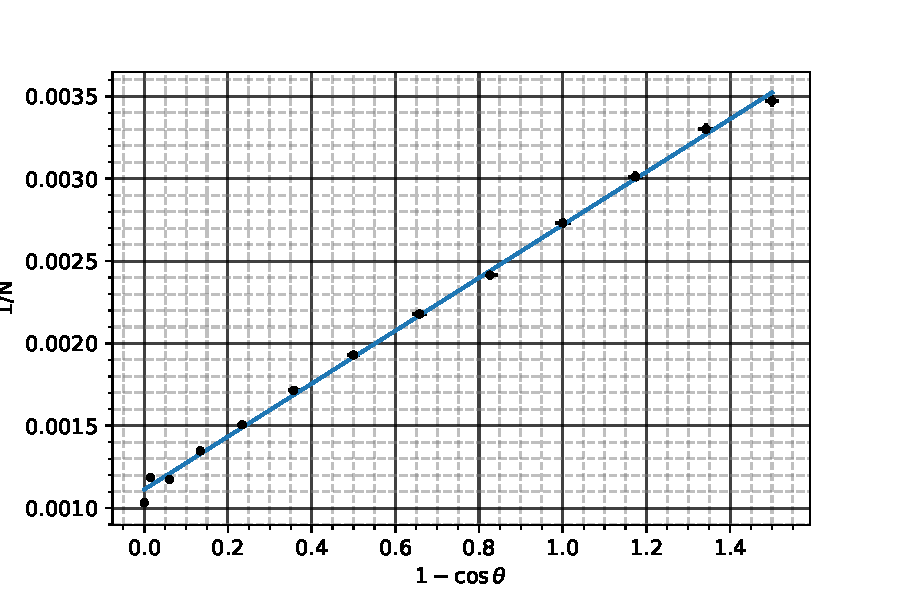
\includegraphics[width=\textwidth]{graph.pdf}
        \caption{График зависимости $\frac{1}{N}(1 - \cos \theta)$}
        \label{fig:graph}
    \end{figure}

    Как видно, эксперементальный график и правда линейный. Пересечение этого графика с осью ординат
    есть наилучшее приближение канала при $\theta = 0$, пересечение графика с прямой $1 - \cos \theta = 1$
    есть наилучшее приближение канала при $\theta = 90^o$. Погрешности данных величин расчитывались исходя из
    погрешностей линеаризации и закона вычисления восвенных погрешностей.

    \begin{center}
        $N_{best}(0) = (898 \pm 13) ~~~ N_{best}(90) = (368 \pm 5)$
    \end{center}

    Возвращаясь обратно к формуле, содержащей энергии фотонов получем при $\theta = 90^o$

    \begin{equation}
        mc^2 \left (\frac{1}{E(90^o)} - \frac{1}{E(0)} \right) = 1
    \end{equation}

    С учетом, что $E(0) = E_{\gamma} = 662$ кэВ можем получить энергию покоя электрона

    \begin{equation}
        mc^2 = E_{\gamma} \frac{N(90^o)}{N(0) - N(90^o)}
    \end{equation}

    Расчитаем погрешность величины $mc^2$. По закону расчета косвенных погрешностей получим

    \begin{equation}
        \sigma_{mc^2} = \sqrt{\left(\frac{\partial (mc^2)}{\partial N(0)} \right)^2 \sigma_{N(0)}^2 + \left(\frac{\partial (mc^2)}{\partial N(90)} \right)^2 \sigma_{N(90)}^2}
    \end{equation}

    \begin{equation}
        \frac{\partial (mc^2)}{\partial N(0)} = \frac{-E_{\gamma} N(90)}{(N(0) - N(90))^2}
    \end{equation}

    \begin{equation}
        \frac{\partial (mc^2)}{\partial N(90)} = \frac{E_{\gamma} N(0)}{(N(0) - N(90))^2}
    \end{equation}

    Полученное значение энергии покоя электрона $mc^2 = (459.65 \pm 15)$ кэВ (погрешност расчитана с учетом того
    что значение $E_{\gamma}$ известно нам точно). Как мы знаем, табличное значение
    энергии покоя электрона $mc^2 = 511$ кэВ, так что, полученное нами значение несколько отличается от табличного.

    \section*{Вывод}

    В данной работе мы исследовали эффект Комптона. Получив линейный график мы убедились в справедливости формулы \eqref{Kompton}, 
    то есть $\gamma$-кваты действительно испытывают рассеяние на свободных частицах, это доказывает корпускулярную
    природу фотонов (эффект Рамзауэра доказывает их полновую природу). По численным значениям мы получили энергию покоя электрона,
    численное значение полученное нами лежит в $3 \sigma$ от реального табличного значения.

\end{document}